\subsection{Medición de la resistencia interna de una fuente} \label{sec:resistencia de fuente}

\paragraph{}
En esta sección se estudió la máxima transferencia de potencia de una fuente con el objetivo de calcular su resistencia interna. Para esto, se montó el circuito de la figura \ref{fig:esq_fuente} utilizando un generador de funciones como fuente.

\begin{figure}[H]
    \centering
    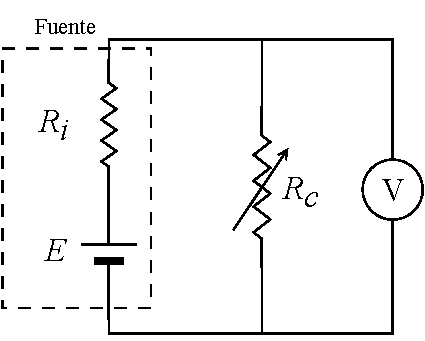
\includegraphics[width = 0.4\linewidth]{Esquemas/Resistencia fuente.pdf}
    \caption{Esquema del circuito eléctrico formado por un generador de funciones con un voltaje constante $E$ y una resistencia interna $R_i$, una resistencia variable $R_C$ y un voltímetro.}
    \label{fig:esq_fuente}
\end{figure}

\paragraph{}
Si se reemplazan las condiciones del circuito en la ecuación \ref{eq_fuente_1}, se obtiene la ecuación \ref{eqn:potencia discipada}, que muestra la potencia total entregada por la fuente en función de la fuente $E$, su resistencia interna $R_i$, y la resistencia variable $R_c$.

\begin{equation}\label{eqn:potencia discipada}
    P_C = \frac{E^2 R_C}{(R_i + R_C)^2}
\end{equation}

\paragraph{}
Se midió la caída de potencial en $R_C$ con el voltímetro conectado en paralelo. A su vez, se midió el valor de $R_C$ en manera independiente. Con estos datos, se realizó un ajuste con la ecuación \ref{eqn:potencia discipada} y se obtuvo el gráfico de la figura \ref{fig:fig_fuente}

\begin{figure}[H]
    \centering
    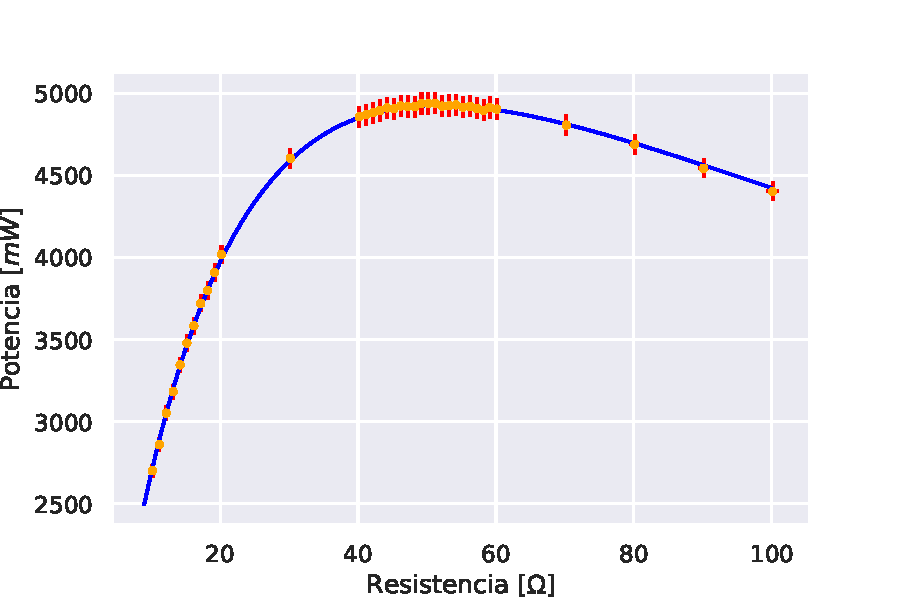
\includegraphics[width = 0.65\linewidth]{figuras/potencia.pdf}    \caption{Ajuste por medio de la ecuación \ref{eqn:potencia discipada} de la potencia en función de la resistencia de carga. Como puede apreciarse, la potencia aumenta con la resistencia hasta un punto, un máximo, el cual representa el valor de la resistencia interna de la fuente. Pasado este punto, la potencia disminuye.}
    \label{fig:fig_fuente}
\end{figure}

\paragraph{}
El máximo de la función que determina la potencia corresponde con el punto donde $R_c$ coincide con $R_i$. Por lo tanto, se encontró dicho máximo y se determinó que la resistencia interna de la fuente es de $R_i=(51,4 \pm 0,5)$$\Omega$. Este resultado es razonable dado que se esperaba que la fuente tenga una resistencia pequeña cuyos efectos sobre el circuito sean despreciables. 